% la-03-vectors.tex

\documentclass[xcolor=dvipsnames]{beamer}
\usepackage{teachbeamer}

\title{Vectors}
\subtitle{{\CourseNumber}, BCIT}

\author{\CourseName}

\date{September 24, 2018}

\begin{document}

\begin{frame}
  \titlepage
\end{frame}

\begin{frame}
  \frametitle{Vectors}
  A vector space $V$ over a field $F$ is a set on which two operations
  (addition and scalar multiplication) are defined. Some axioms need
  to be fulfilled, most relevantly \alert{closure} with respect to
  addition and scalar multiplication:
  \begin{itemize}
  \item If $v,w\in{}V$, then $v+w\in{}V$
  \item If $a\in{}F,v\in{}V$, then $av\in{}V$
  \end{itemize}
  In this course, the field will always be $\mathbb{R}$ or
  $\mathbb{C}$, the real or the complex numbers.
\end{frame}

\begin{frame}
  \frametitle{Excursus: Complex Numbers}
  The following set
  \begin{equation}
    \label{eq:oiphaebo}
    \mathbb{C}=\{a+bi|a,b\in\mathbb{R}\}
  \end{equation}
  is called the set of complex numbers. Note that
  $\mathbb{R}\subset\mathbb{C}$. Operations (addition, multiplication,
  and so on) are defined on complex numbers the same way as on real
  numbers with one additional rule:
  \begin{equation}
    \label{eq:thaikiec}
    i^{2}=-1
  \end{equation}
\end{frame}

\begin{frame}
  \frametitle{Excursus: Complex Operators}
  {\ubung} Find the determinant of the following matrix:
  \begin{equation}
    \label{eq:ohhohhoo}
    A=\left[
      \begin{array}{cc}
        1-4i & 3-i \\
        -3i & 3+4i
      \end{array}\right]
  \end{equation}
{\ubung} A matrix that equals its conjugate transpose is called a
\alert{Hermitian matrix}. Calculate the determinate of the following
example.
\begin{equation}
  \label{eq:ohsaiphi}
  B=\left[
    \begin{array}{ccc}
      2 & 2+i & 4 \\
      2-i & 3 & i \\
      4 & -i & 1
    \end{array}\right]
\end{equation}
{\ubung} Use expansion by conjugates to divide
\begin{equation}
  \label{eq:choomeux}
  \frac{7-2i}{3+4i}
\end{equation}
\end{frame}

\begin{frame}
  \frametitle{Excursus: Polar Form}
  The complex numbers correspond to vectors in $\mathbb{R}^{2}$.
    \begin{figure}[h]
    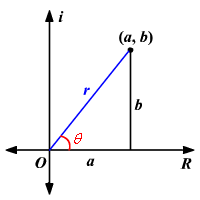
\includegraphics[scale=0.32]{./diagrams/polar.png}
  \end{figure}
Instead of providing the coordinates $(a,b)$ of a complex number, it
is sometimes useful to provide the \alert{polar form} $(r,\theta)$.
\begin{equation}
  \label{eq:eekaerai}
  \begin{array}{ll}
    a=r\cos\theta & b=r\sin\theta \\
    r^{2}=a^{2}+b^{2} & \tan\theta=\frac{b}{a}
  \end{array}
\end{equation}
A complex number $a+bi$ can always be written in its polar form $a+bi=r(\cos\theta+i\sin\theta)$.
\end{frame}

\begin{frame}
  \frametitle{Excursus: Euler's Formula}
  One of the most famous formulas in mathematics is Euler's formula
  \begin{equation}
    \label{eq:kiagaiga}
    e^{ix}=\cos{}x+i\sin{}x
  \end{equation}
For the proof, we need some calculus. Recall the Maclaurin series
expansions
\begin{equation}
  \label{eq:uthairoj}
  e^{x}=\sum_{j=0}^{\infty}\frac{x^{j}}{j!}
\end{equation}
\begin{equation}
  \label{eq:eepiewez}
  \cos{}x=\sum_{j=0}^{\infty}(-1)^{j}\frac{x^{2j}}{(2j)!}
\end{equation}
\begin{equation}
  \label{eq:mohhaich}
  \sin{}x=\sum_{j=0}^{\infty}(-1)^{j}\frac{x^{2j+1}}{(2j+1)!}
\end{equation}
Calculus still works in the complex numbers, now try to find $e^{ix}$. 
\end{frame}

\begin{frame}
  \frametitle{Excursus: Use of the Polar Form}
Euler's formula makes multiplication, division, exponentiation and
finding roots of complex numbers in polar form more simple.

\medskip

{\ubung} Multiply $(4,60^{\circ})$ by $(2,20^{\circ})$, where the
given factors are complex numbers provided in polar form.

\medskip

{\ubung} Divide $(8,100^{\circ})$ by $(4,65^{\circ})$, where the
given numbers are complex numbers provided in polar form.

\medskip

{\ubung} Find, using two alternative ways,
\begin{equation}
  \label{eq:iekaekep}
  \frac{-2+5i}{-1-i}\mbox{ and }\left(2+3i\right)^{5}
\end{equation}
\end{frame}

\begin{frame}
  \frametitle{Excursus: Closeted Functions}
You may remember that I once called trigonometric functions ``closeted
exponential functions.'' Here is the reason. Consider
\begin{equation}
  \label{eq:eixeivei}
  \begin{array}{rcl}
  e^{ix}&=&\cos{}x+i\sin{}x \\
  e^{-ix}&=&\cos{}x-i\sin{}x
  \end{array}
\end{equation}
Add and subtract these two equations for
\begin{equation}
  \label{eq:ohrayaxu}
  \cos{}x=\frac{e^{ix}+e^{-ix}}{2}
\end{equation}
\begin{equation}
  \label{eq:quuiquei}
  \sin{}x=\frac{e^{ix}-e^{-ix}}{2i}
\end{equation}
This is the definition of trigonometric functions on $\mathbb{C}$. The
hyperbolic trigonometric functions are closeted sines and cosines,
since $\cosh(x)=\cos(ix)$ and $i\sinh(x)=\sin(ix)$. 
\end{frame}

\begin{frame}
  \frametitle{Excursus: de Moivre's Formula}
\begin{block}{de Moivre's Formula}
  $\left(re^{i\theta}\right)^{n}=r^{n}e^{in\theta}$
\end{block}

\medskip

\beispiel{Cube Roots} Find the solution set for the following equation
and $c=(27,120^{\circ})$, where $c$ is a complex number provided in
polar form.
\begin{equation}
  \label{eq:aephacha}
  x^{3}=c
\end{equation}

\medskip

By de Moivre's formula, $x=(3,40^{\circ})$ is a solution. However,
$c=(27,480^{\circ})$ and therefore, by de Moivre's formula again,
$x=(3,160^{\circ})$ is also a solution. $c=(27,840^{\circ})$ provides
the third solution, $x=(3,280^{\circ})$. Polynomial equations of
degree $n$ always have $n$ solutions in $\mathbb{C}$. 
\end{frame}

\begin{frame}
  \frametitle{Excursus: Complex Roots}
    \begin{figure}[h]
    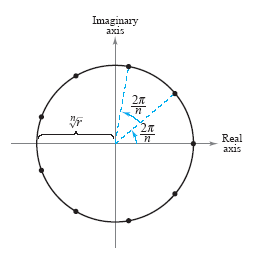
\includegraphics[scale=0.5]{./diagrams/comproot.png}
  \end{figure}
  {\ubung} Solve the equation
  \begin{equation}
    \label{eq:phoojahs}
    x^{2}+4x+5=0
  \end{equation}
  in the complex numbers.
\end{frame}

\begin{frame}
  \frametitle{Excursus: Casus Irreducibilis}
  What is the use of complex numbers? There are many engineering
  examples, but here is one from solving cubic equations. Find the
  solutions for
  \begin{equation}
    \label{eq:oozaechi}
    x^{3}-3x+1=0
  \end{equation}
  Cardano's formula gives us the three solutions,
  \begin{equation}
    \label{eq:iejopice}
    x_{k}=w_{k}\sqrt[3]{-\frac{1}{2}+\sqrt{\frac{-3}{4}}}+w_{k}^{2}\sqrt[3]{-\frac{1}{2}-\sqrt{\frac{-3}{4}}}
  \end{equation}
  where $k=1,2,3$ and $(w_{1},w_{2},w_{3})$ are the three cube roots
  of $1$. You can look up online why Cardano's formula is true. The
  point is that all the solutions to this problem are real numbers,
  but we have to use complex algebra to calculate them.
\end{frame}

\begin{frame}
  \frametitle{Linear Combination and Span}
  If $T=\{v_{1},{\ldots},v_{k}\}$ is a set of vectors and
  $\{x_{1},{\ldots},x_{k}\}\subset{}F$ is a set of scalars, then
  \begin{equation}
    \label{eq:aiveatah}
    x_{1}v_{1}+{\ldots}+x_{k}v_{k}
  \end{equation}
  is called a \alert{linear combination} of $v_{1},{\ldots},v_{k}$.
  The set of all linear combinations of $v_{1},{\ldots},v_{k}$ is
  called the \alert{span} of $v_{1},{\ldots},v_{k}$.

  \medskip

  The span of a set of vectors is a \alert{subspace} of $V$, meaning
  that it is closed with respect to addition and scalar
  multiplication. The solution set for a system of linear equations is
  always a subspace (if $u,v\in{}S$ and $a\in{}F$, then $u+v\in{}S$
  and $au\in{}S$).
\end{frame}

\begin{frame}
  \frametitle{Linear Independence}
  A set of vectors $v_{1},{\ldots},v_{k}$ is \alert{linearly
    independent} if and only if the vector equation
  \begin{equation}
    \label{eq:wohsiete}
    x_{1}v_{1}+{\ldots}+x_{k}v_{k}=0    
  \end{equation}
  has the unique solution $(x_{1},{\ldots},x_{k})=(0,{\ldots},0)$.
\end{frame}

\begin{frame}
  \frametitle{Theorems of Linear Independence}
  \begin{enumerate}
  \item $v_{1},{\ldots},v_{k}$ are linearly dependent if and only if
    at least one of these vectors is a linear combination of the
    others
  \item The columns of a matrix $A$ are linearly independent if and
    only if the rank of $A$ is $k$ (the number of columns).
  \item A square matrix is invertible if and only if its columns (or
    rows) are linearly independent.
  \end{enumerate}
\end{frame}

\begin{frame}
  \frametitle{Basis and Dimension}
  If $V$ is a vector space, then the set $B=\{b_{1},{\ldots},b_{k}\}$
  is a \alert{basis} of $V$ if and only if $v_{1},{\ldots},v_{k}$ are linearly
  independent and the span of $B$ is $V$.
  \begin{block}{Unique Representation}
    Every vector $u\in{}V$ is a linear combination
    $u=x_{1}b_{1}+{\ldots}+x_{k}b_{k}$ of basis vectors, if such a basis
    exists. The ordered set $(x_{1},{\ldots},x_{k})$ is called the
    \alert{coordinates} of $u$ with respect to basis $B$. 
  \end{block}
  There is a theorem that tells us that if two sets of vectors $B_{1}$
  and $B_{2}$ are bases of vector space $V$, then the cardinality of
  $B_{1}$ equals the cardinality of $B_{2}$. Thus, if a finite base
  exists, it makes sense to define the \alert{dimension} of the vector
  space to be the cardinality of that base.
\end{frame}

\begin{frame}
  \frametitle{Vector Spaces}
  A finite-dimensional vector space (let the dimension be $n$) over
  the real numbers corresponds to a set of ordered sets of real
  numbers (the coordinates of the vectors). In other words, it
  corresponds to $\mathbb{R}^{n}$. 

\medskip

Examples of vector spaces:
\begin{itemize}
\item three-dimensional space $\mathbb{R}^{3}$
\item the set of all straight lines in two-dimensional space
\item the set of all parabolas in two-dimensional space
\item the set of all circles in two-dimensional space
\item the set of all polynomials with degree $k\leq{}n$
\item the set of all real-valued functions on $\mathbb{R}$
\end{itemize}
Try to determine the dimensions of these vector spaces.
\end{frame}

\begin{frame}
  \frametitle{Displacement Vectors}
  One way to interpret a vector in $\mathbb{R}^{2}$ or
  $\mathbb{R}^{3}$ is to make it refer to a point in the
  $xy$-plane or $xyz$-three-dimensional space. The usual
  interpretation, however, is as a \alert{displacement vector} with a
  direction and a length. Here is an example:
  \begin{equation}
    \label{eq:lapheeka}
    \vec{v}=\left(
    \begin{array}{c}
      3 \\
      5 \\
      -1
    \end{array}\right)
  \end{equation}
\end{frame}

\begin{frame}
  \frametitle{Vector Algebra}
  Vectors can be added, subtracted, and multiplied by a scalar (a real
  number).
  \begin{equation}
    \label{eq:kaepuema}
    \left(
    \begin{array}{c}
      3 \\
      5 \\
      -1
    \end{array}\right)+
  \left(
    \begin{array}{c}
      2 \\
      \pi \\
      -6
    \end{array}\right)=
  \left(
    \begin{array}{c}
      5 \\
      5+\pi \\
      -7
    \end{array}\right)
  \end{equation}
  \begin{equation}
    \label{eq:kemodaim}
    1.5\cdot\left(
    \begin{array}{c}
      3 \\
      5 \\
      -1
    \end{array}\right)=
  \left(
    \begin{array}{c}
      4.5 \\
      7.5 \\
      -1.5
    \end{array}\right)
  \end{equation}
\end{frame}

\begin{frame}
  \frametitle{Unit Vectors}
  All three-dimensional vectors can be expressed in components. For
  this expression we need unit vectors. Any three linearly independent
  vectors would work, but it makes sense to use the following three:
  \begin{equation}
    \label{eq:bahniech}
    \vec{i}=\left(
    \begin{array}{c}
      1 \\
      0 \\
      0
    \end{array}\right)\hspace{.2in}
    \vec{j}=\left(
    \begin{array}{c}
      0 \\
      1 \\
      0
    \end{array}\right)\hspace{.2in}
    \vec{k}=\left(
    \begin{array}{c}
      0 \\
      0 \\
      1
    \end{array}\right)
  \end{equation}
\end{frame}

\begin{frame}
  \frametitle{Vector Decomposition}
  For any vector $\vec{v}$  (assuming from now on three dimensions),
  \begin{equation}
    \label{eq:teequahg}
    \vec{v}=v_{x}\vec{i}+v_{y}\vec{j}+v_{z}\vec{k}
  \end{equation}
where $V=(v_{x},v_{y},v_{z})$, and $V$ is the point to which the
origin $O=(0,0,0)$ would be displaced by vector
\begin{equation}
  \label{eq:zaegiexo}
  \vec{v}=\left(
    \begin{array}{c}
      v_{x} \\
      v_{y} \\
      v_{z} \\
    \end{array}\right)
\end{equation}
\end{frame}

\begin{frame}
  \frametitle{Vector Length and Distance Between Two Points}
  The length of vector $\vec{v}$ is
  \begin{equation}
    \label{eq:ogeithie}
    \Vert\vec{v}\Vert=\sqrt{v_{x}^{2}+v_{y}^{2}+v_{z}^{2}}
  \end{equation}
The distance between two points $P$ and $Q$ is the length of a
displacement vector between them. Let $\vec{OP}$ be the displacement
vector from $O$ to $P$ and so on. Then
\begin{equation}
  \label{eq:ahnoocae}
  \vec{PQ}=\vec{PO}+\vec{OQ}=\vec{OQ}-\vec{OP}
\end{equation}
and $\Vert\vec{PQ}\Vert$ is the distance between $P$ and $Q$.
\end{frame}

\begin{frame}
  \frametitle{Dot Product}
  The following two definition of the \alert{dot product}, or
  \alert{scalar product}, $\vec{v}\cdot\vec{w}$ are equivalent:
  \begin{description}
  \item[geometric]
    $\vec{v}\cdot\vec{w}=\Vert\vec{v}\Vert\cdot\Vert\vec{w}\Vert\cdot\cos\vartheta$
    where $\vartheta$ is the angle between $\vec{v}$ and $\vec{w}$,
    $0\leq\vartheta\leq\pi$.
  \item[algebraic] $\vec{v}\cdot\vec{w}=v_{x}w_{x}+v_{y}w_{y}+v_{z}w_{z}$
  \end{description}
The dot product is a number, not a vector.
\end{frame}

\begin{frame}
  \frametitle{Dot Product}
  Now we need to show that the two definitions are equivalent.
  Consider a triangle $PQR$ in three-dimensional space. Let
  $\vec{v}=\vec{PQ},\vec{w}=\vec{PR}$. Then
  \begin{equation}
    \label{eq:oobeipho}
  \vec{QR}=\vec{QP}+\vec{PR}=-\vec{v}+\vec{w}=\vec{w}-\vec{v}  
\end{equation}
Here is the law of cosines for this triangle:
\begin{equation}
  \label{eq:aiwahzoa}
  \Vert\vec{w}-\vec{v}\Vert^{2}=\Vert\vec{v}\Vert^{2}+\Vert\vec{w}\Vert^{2}-2\Vert\vec{v}\Vert\cdot\Vert\vec{w}\Vert\cos\vartheta
\end{equation}
It follows that the two definitions are equivalent.
\end{frame}

\begin{frame}
  \frametitle{Dot Product}
\begin{block}{Perpendicularity and Dot Product}
  Two non-zero vectors $\vec{v}$ and $\vec{w}$ are perpendicular, or
  orthogonal, if and only if $\vec{v}\cdot\vec{w}=0$.
\end{block}

\bigskip

\begin{block}{Magnitude and Dot Product}
  Magnitude and dot product are related as follows: $\vec{v}\cdot\vec{v}=\Vert\vec{v}\Vert$.
\end{block}
\end{frame}

% this is NOT correct
% \begin{frame}
%   \frametitle{Dot Product Exercise}
%   {\ubung} Find a normal vector to the following planes (a normal vector to a
%   plane is perpendicular to all non-zero vectors displacing points on
%   the plane).
%   \begin{equation}
%     \label{eq:afanaagu}
%     2x+y-z=5
%   \end{equation}
%   \begin{equation}
%     \label{eq:reeregha}
%     2(x-z)=3(x+y)
%   \end{equation}
%   For (\ref{eq:afanaagu}), set $x=1,y=1$, then $z=-2$ for
%   $P=(1,1,-2)$. Then set $x=3,y=1$, so $z=2$ for $Q=(3,1,2)$. Both $P$
%   and $Q$ are on the plane, so $\vec{PQ}=\vec{OQ}-\vec{OP}$ is a
%   vector displacing two points in the plane. To find a vector
%   perpendicular to it consider the dot product
% \begin{equation}
%   \label{eq:chiemaig}
%   -2x+0y-4z=0
% \end{equation}
% Choose $x=1,y=1$, so $z=-0.5$. The vector
% $1\cdot\vec{i}+1\cdot\vec{j}-0.5\cdot\vec{k}$ is a normal vector to the
% plane $2x+y-z=5$.
% \end{frame}

\begin{frame}
  \frametitle{Dot Product Exercise}
  {\ubung} Find the angle between
  \begin{equation}
    \label{eq:tauhohju}
    \vec{v}=\left(
      \begin{array}{c}
        4 \\
        0 \\
        7
      \end{array}\right)\hspace{.5in}\vec{w}=\left(
      \begin{array}{c}
        -2 \\
        1 \\
        3
      \end{array}\right)
  \end{equation}
  Consider the dot product
  \begin{equation}
    \label{eq:ijaquahd}
    4\cdot(-2)+0\cdot{}1+7\cdot{}3=13
  \end{equation}
According to the two equivalent definitions of the dot product, this
is equal to
\begin{equation}
  \label{eq:ohyizaeb}
  \Vert\vec{v}\Vert\cdot\Vert\vec{w}\Vert\cdot\cos\vartheta=\sqrt{4^{2}+7^{2}}\cdot\sqrt{(-2)^{2}+1^{2}+3^{2}}\cdot\cos\vartheta
\end{equation}
Therefore,
\begin{equation}
  \label{eq:yohsheen}
  \vartheta=\arccos\frac{13}{\sqrt{4^{2}+7^{2}}\cdot\sqrt{(-2)^{2}+1^{2}+3^{2}}}=64.47^{\circ}
\end{equation}
\end{frame}

\begin{frame}
  \frametitle{Planes Again}
  The equation of the plane with normal vector
  $\vec{n}=a\vec{i}+b\vec{j}+c\vec{k}$ and containing the point
  $P=(x_{0},y_{0},z_{0})$ is
  \begin{equation}
    \label{eq:ijaeriri}
    a(x-x_{0})+b(y-y_{0})+c(z-z_{0})=0
  \end{equation}
  Alternatively, for $d=ax_{0}+by_{0}+cz_{0}$
  \begin{equation}
    \label{eq:bamoyeez}
    ax+by+cz=d
  \end{equation}
\end{frame}

\begin{frame}
  \frametitle{Cross Product}
  \begin{figure}[h]
    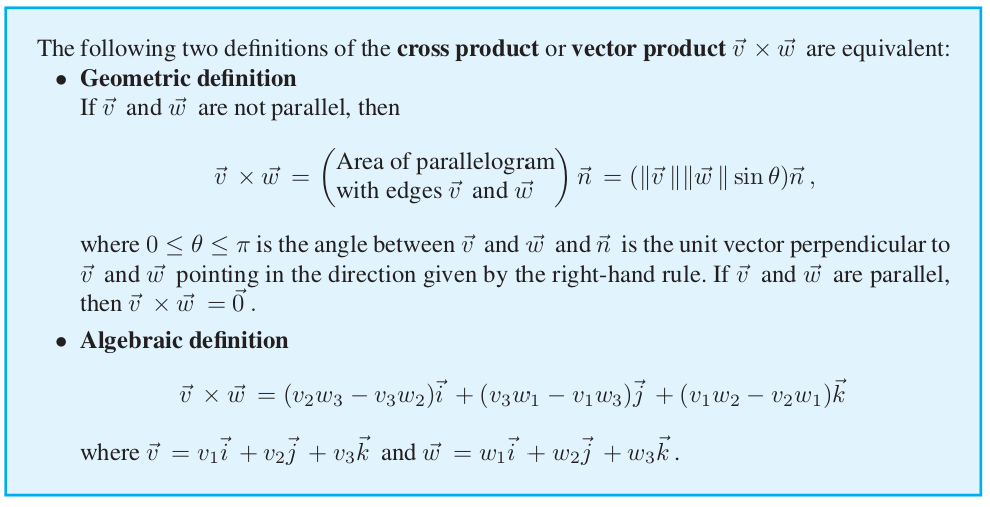
\includegraphics[scale=0.32]{./diagrams/crossproduct.png}
  \end{figure}
\end{frame}

\begin{frame}
  \frametitle{Cross Product}
  If you know what a determinant is, you can remember the algebraic
  definition as follows.
  \begin{equation}
    \label{eq:abeekohc}
    \vec{v}\times\vec{w}=\left\vert
      \begin{array}{ccc}
        \vec{i} & \vec{j} & \vec{k} \\
        v_{1} & v_{2} & v_{3} \\
        w_{1} & w_{2} & w_{3}
      \end{array}\right\vert
  \end{equation}
  Note that $\vec{w}\times\vec{v}=-\vec{v}\times\vec{w}$.
\end{frame}

\begin{frame}
  \frametitle{Cross Product Exercise}
  {\ubung} Use the cross product to find the linear equation containing the
  three points
  \begin{equation}
    \label{eq:eiyeigaz}
    \begin{array}{rcl}
      P&=&(1,3,0) \\
      Q&=&(3,4,-3) \\
      R&=&(3,6,2)
    \end{array}
  \end{equation}
\end{frame}

\begin{frame}
  \frametitle{Cross Product Exercise Answer}
One way to find the answer to the last exercise (without using the
cross product) is to solve the following system of linear equations
for the plane $x+ay+bz=c$,
\begin{equation}
  \label{eq:yohghaef}
  \begin{array}{rcl}
    1+3a+0b&=&c \\
    3+4a-3b&=&c \\
    3+6a+2b&=&c
  \end{array}
\end{equation}
Change this to
\begin{equation}
  \label{eq:oxeingiu}
  \begin{array}{rcl}
    3a+0b-c&=&-1 \\
    4a-3b-c&=&-3 \\
    6a+2b-c&=&-3 \\
  \end{array}
\end{equation}
Using matrices,
\begin{equation}
  \label{eq:ukohjiej}
  \left(
    \begin{array}{ccc}
      3&0&-1 \\
      4&-3&-1 \\
      6&2&-1
    \end{array}\right)\cdot\left(
    \begin{array}{c}
      a \\
      b \\
      c
    \end{array}\right)=\left(
    \begin{array}{c}
      -1 \\
      -3 \\
      -3
    \end{array}\right)
\end{equation}
\end{frame}

\begin{frame}
  \frametitle{Cross Product Exercise Answer}
  Equation (\ref{eq:ukohjiej}) yields the solution
  \begin{equation}
    \label{eq:maeshael}
      x-\frac{10}{11}y+\frac{4}{11}z=-\frac{19}{11}
  \end{equation}
Now let's use the cross product instead, avoiding the matrices. Note
that
\begin{equation}
  \label{eq:ushahroh}
  \begin{array}{rcl}
    \vec{PQ}&=&2\vec{i}+\vec{j}-3\vec{k} \\
    \vec{PR}&=&2\vec{i}+3\vec{j}+2\vec{k}
  \end{array}
\end{equation}
The cross product, using the algebraic definition, is
$\vec{u}=\vec{PQ}\times\vec{PR}=11\vec{i}-10\vec{j}+4\vec{k}$.
\end{frame}

\begin{frame}
  \frametitle{Cross Product Exercise Answer}
  Let $P=(x_{0},y_{0},z_{0})$ be a fixed point on the plane with known
  coordinates. Since any point $S=(x,y,z)$ on the plane fulfills
\begin{equation}
  \label{eq:iefeeboh}
  \vec{PS}\cdot\vec{u}=0
\end{equation}
this can be turned into the plane equation
\begin{equation}
  \label{eq:vetiexup}
  u_{x}(x-x_{0})+u_{y}(y-y_{0})+u_{z}(z-z_{0})=0
\end{equation}
Therefore, using $P=(1,3,0)$, this translates into
\begin{equation}
  \label{eq:eechawoi}
11x-10y+4z=19  
\end{equation}
which is equivalent to (\ref{eq:maeshael}). Notice how easy it is to
find a linear equation when you have a point $P=(x_{0},y_{0},z_{0})$
on the plane and a normal vector $\vec{u}$ to the plane
$u_{x}\vec{i}+u_{y}\vec{j}+u_{z}\vec{k}$:
\begin{equation}
  \label{eq:quaghoob}
u_{x}x+u_{y}y+u_{z}z=u_{x}x_{0}+u_{y}y_{0}+u_{z}z_{0}
\end{equation}
\end{frame}

\begin{frame}
  \frametitle{Exercise}
  {\ubung} Find all interior angles for and the plane equation
  containing the triangle with points
  \begin{equation}
    \label{eq:yeibieba}
    P=(1,4,-2),Q=(-1,1,2),R=(-1,3,1)
  \end{equation}
\end{frame}

\begin{frame}
  \frametitle{Exercise}
  {\ubung} Find the equation of the tangent plane with respect to the
  unit circle at $P=(0.2,0.3,\sqrt{0.87})$.

  \medskip

  Hint: identify a vector that is orthogonal to the plane or use
  partial derivatives for the function whose function graph overlaps
  with the relevant part of the sphere.
\end{frame}

\begin{frame}
  \frametitle{End of Lesson}
Next Lesson: Least Squares Approximation
\end{frame}

\end{document}

